\documentclass[]{book}
\usepackage{lmodern}
\usepackage{amssymb,amsmath}
\usepackage{ifxetex,ifluatex}
\usepackage{fixltx2e} % provides \textsubscript
\ifnum 0\ifxetex 1\fi\ifluatex 1\fi=0 % if pdftex
  \usepackage[T1]{fontenc}
  \usepackage[utf8]{inputenc}
\else % if luatex or xelatex
  \ifxetex
    \usepackage{mathspec}
  \else
    \usepackage{fontspec}
  \fi
  \defaultfontfeatures{Ligatures=TeX,Scale=MatchLowercase}
\fi
% use upquote if available, for straight quotes in verbatim environments
\IfFileExists{upquote.sty}{\usepackage{upquote}}{}
% use microtype if available
\IfFileExists{microtype.sty}{%
\usepackage{microtype}
\UseMicrotypeSet[protrusion]{basicmath} % disable protrusion for tt fonts
}{}
\usepackage[margin=1in]{geometry}
\usepackage{hyperref}
\hypersetup{unicode=true,
            pdftitle={Sleep quality analysis},
            pdfauthor={Arturo Laflor},
            pdfborder={0 0 0},
            breaklinks=true}
\urlstyle{same}  % don't use monospace font for urls
\usepackage{natbib}
\bibliographystyle{apalike}
\usepackage{color}
\usepackage{fancyvrb}
\newcommand{\VerbBar}{|}
\newcommand{\VERB}{\Verb[commandchars=\\\{\}]}
\DefineVerbatimEnvironment{Highlighting}{Verbatim}{commandchars=\\\{\}}
% Add ',fontsize=\small' for more characters per line
\usepackage{framed}
\definecolor{shadecolor}{RGB}{248,248,248}
\newenvironment{Shaded}{\begin{snugshade}}{\end{snugshade}}
\newcommand{\KeywordTok}[1]{\textcolor[rgb]{0.13,0.29,0.53}{\textbf{{#1}}}}
\newcommand{\DataTypeTok}[1]{\textcolor[rgb]{0.13,0.29,0.53}{{#1}}}
\newcommand{\DecValTok}[1]{\textcolor[rgb]{0.00,0.00,0.81}{{#1}}}
\newcommand{\BaseNTok}[1]{\textcolor[rgb]{0.00,0.00,0.81}{{#1}}}
\newcommand{\FloatTok}[1]{\textcolor[rgb]{0.00,0.00,0.81}{{#1}}}
\newcommand{\ConstantTok}[1]{\textcolor[rgb]{0.00,0.00,0.00}{{#1}}}
\newcommand{\CharTok}[1]{\textcolor[rgb]{0.31,0.60,0.02}{{#1}}}
\newcommand{\SpecialCharTok}[1]{\textcolor[rgb]{0.00,0.00,0.00}{{#1}}}
\newcommand{\StringTok}[1]{\textcolor[rgb]{0.31,0.60,0.02}{{#1}}}
\newcommand{\VerbatimStringTok}[1]{\textcolor[rgb]{0.31,0.60,0.02}{{#1}}}
\newcommand{\SpecialStringTok}[1]{\textcolor[rgb]{0.31,0.60,0.02}{{#1}}}
\newcommand{\ImportTok}[1]{{#1}}
\newcommand{\CommentTok}[1]{\textcolor[rgb]{0.56,0.35,0.01}{\textit{{#1}}}}
\newcommand{\DocumentationTok}[1]{\textcolor[rgb]{0.56,0.35,0.01}{\textbf{\textit{{#1}}}}}
\newcommand{\AnnotationTok}[1]{\textcolor[rgb]{0.56,0.35,0.01}{\textbf{\textit{{#1}}}}}
\newcommand{\CommentVarTok}[1]{\textcolor[rgb]{0.56,0.35,0.01}{\textbf{\textit{{#1}}}}}
\newcommand{\OtherTok}[1]{\textcolor[rgb]{0.56,0.35,0.01}{{#1}}}
\newcommand{\FunctionTok}[1]{\textcolor[rgb]{0.00,0.00,0.00}{{#1}}}
\newcommand{\VariableTok}[1]{\textcolor[rgb]{0.00,0.00,0.00}{{#1}}}
\newcommand{\ControlFlowTok}[1]{\textcolor[rgb]{0.13,0.29,0.53}{\textbf{{#1}}}}
\newcommand{\OperatorTok}[1]{\textcolor[rgb]{0.81,0.36,0.00}{\textbf{{#1}}}}
\newcommand{\BuiltInTok}[1]{{#1}}
\newcommand{\ExtensionTok}[1]{{#1}}
\newcommand{\PreprocessorTok}[1]{\textcolor[rgb]{0.56,0.35,0.01}{\textit{{#1}}}}
\newcommand{\AttributeTok}[1]{\textcolor[rgb]{0.77,0.63,0.00}{{#1}}}
\newcommand{\RegionMarkerTok}[1]{{#1}}
\newcommand{\InformationTok}[1]{\textcolor[rgb]{0.56,0.35,0.01}{\textbf{\textit{{#1}}}}}
\newcommand{\WarningTok}[1]{\textcolor[rgb]{0.56,0.35,0.01}{\textbf{\textit{{#1}}}}}
\newcommand{\AlertTok}[1]{\textcolor[rgb]{0.94,0.16,0.16}{{#1}}}
\newcommand{\ErrorTok}[1]{\textcolor[rgb]{0.64,0.00,0.00}{\textbf{{#1}}}}
\newcommand{\NormalTok}[1]{{#1}}
\usepackage{longtable,booktabs}
\usepackage{graphicx,grffile}
\makeatletter
\def\maxwidth{\ifdim\Gin@nat@width>\linewidth\linewidth\else\Gin@nat@width\fi}
\def\maxheight{\ifdim\Gin@nat@height>\textheight\textheight\else\Gin@nat@height\fi}
\makeatother
% Scale images if necessary, so that they will not overflow the page
% margins by default, and it is still possible to overwrite the defaults
% using explicit options in \includegraphics[width, height, ...]{}
\setkeys{Gin}{width=\maxwidth,height=\maxheight,keepaspectratio}
\IfFileExists{parskip.sty}{%
\usepackage{parskip}
}{% else
\setlength{\parindent}{0pt}
\setlength{\parskip}{6pt plus 2pt minus 1pt}
}
\setlength{\emergencystretch}{3em}  % prevent overfull lines
\providecommand{\tightlist}{%
  \setlength{\itemsep}{0pt}\setlength{\parskip}{0pt}}
\setcounter{secnumdepth}{5}
% Redefines (sub)paragraphs to behave more like sections
\ifx\paragraph\undefined\else
\let\oldparagraph\paragraph
\renewcommand{\paragraph}[1]{\oldparagraph{#1}\mbox{}}
\fi
\ifx\subparagraph\undefined\else
\let\oldsubparagraph\subparagraph
\renewcommand{\subparagraph}[1]{\oldsubparagraph{#1}\mbox{}}
\fi

%%% Use protect on footnotes to avoid problems with footnotes in titles
\let\rmarkdownfootnote\footnote%
\def\footnote{\protect\rmarkdownfootnote}

%%% Change title format to be more compact
\usepackage{titling}

% Create subtitle command for use in maketitle
\newcommand{\subtitle}[1]{
  \posttitle{
    \begin{center}\large#1\end{center}
    }
}

\setlength{\droptitle}{-2em}
  \title{Sleep quality analysis}
  \pretitle{\vspace{\droptitle}\centering\huge}
  \posttitle{\par}
  \author{Arturo Laflor}
  \preauthor{\centering\large\emph}
  \postauthor{\par}
  \predate{\centering\large\emph}
  \postdate{\par}
  \date{2017-04-17}

\usepackage{booktabs}
\usepackage{amsthm}
\usepackage{multirow}
\usepackage{multicol}
\usepackage{float}
\makeatletter
\def\thm@space@setup{%
  \thm@preskip=8pt plus 2pt minus 4pt
  \thm@postskip=\thm@preskip
}
\makeatother

\begin{document}
\maketitle

{
\setcounter{tocdepth}{1}
\tableofcontents
}
\chapter{Prerequisites}\label{prerequisites}

This is a \emph{sample} book written in \textbf{Markdown}. You can use
anything that Pandoc's Markdown supports, e.g., a math equation
\(a^2 + b^2 = c^2\).

For now, you have to install the development versions of
\textbf{bookdown} from Github:

\begin{Shaded}
\begin{Highlighting}[]
\NormalTok{devtools::}\KeywordTok{install_github}\NormalTok{(}\StringTok{"rstudio/bookdown"}\NormalTok{)}
\end{Highlighting}
\end{Shaded}

Remember each Rmd file contains one and only one chapter, and a chapter
is defined by the first-level heading \texttt{\#}.

To compile this example to PDF, you need to install XeLaTeX.

\chapter{Introduction}\label{intro}

You can label chapter and section titles using \texttt{\{\#label\}}
after them, e.g., we can reference Chapter \ref{intro}. If you do not
manually label them, there will be automatic labels anyway, e.g.,
Chapter \ref{methods}.

Figures and tables with captions will be placed in \texttt{figure} and
\texttt{table} environments, respectively.

\begin{Shaded}
\begin{Highlighting}[]
\KeywordTok{par}\NormalTok{(}\DataTypeTok{mar =} \KeywordTok{c}\NormalTok{(}\DecValTok{4}\NormalTok{, }\DecValTok{4}\NormalTok{, .}\DecValTok{1}\NormalTok{, .}\DecValTok{1}\NormalTok{))}
\KeywordTok{plot}\NormalTok{(pressure, }\DataTypeTok{type =} \StringTok{'b'}\NormalTok{, }\DataTypeTok{pch =} \DecValTok{19}\NormalTok{)}
\end{Highlighting}
\end{Shaded}

\begin{figure}

{\centering 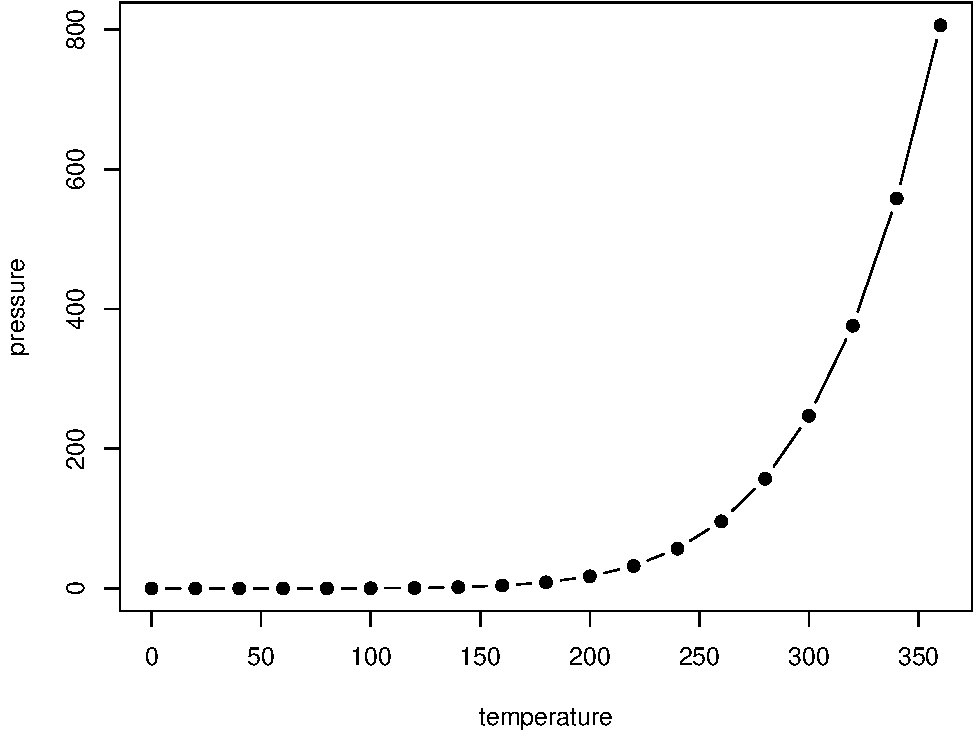
\includegraphics[width=0.8\linewidth]{bookdown-demo_files/figure-latex/nice-fig-1} 

}

\caption{Here is a nice figure!}\label{fig:nice-fig}
\end{figure}

Reference a figure by its code chunk label with the \texttt{fig:}
prefix, e.g., see Figure \ref{fig:nice-fig}. Similarly, you can
reference tables generated from \texttt{knitr::kable()}, e.g., see Table
\ref{tab:nice-tab}.

\begin{Shaded}
\begin{Highlighting}[]
\NormalTok{knitr::}\KeywordTok{kable}\NormalTok{(}
  \KeywordTok{head}\NormalTok{(iris, }\DecValTok{20}\NormalTok{), }\DataTypeTok{caption =} \StringTok{'Here is a nice table!'}\NormalTok{,}
  \DataTypeTok{booktabs =} \OtherTok{TRUE}
\NormalTok{)}
\end{Highlighting}
\end{Shaded}

\begin{table}

\caption{\label{tab:nice-tab}Here is a nice table!}
\centering
\begin{tabular}[t]{rrrrl}
\toprule
Sepal.Length & Sepal.Width & Petal.Length & Petal.Width & Species\\
\midrule
5.1 & 3.5 & 1.4 & 0.2 & setosa\\
4.9 & 3.0 & 1.4 & 0.2 & setosa\\
4.7 & 3.2 & 1.3 & 0.2 & setosa\\
4.6 & 3.1 & 1.5 & 0.2 & setosa\\
5.0 & 3.6 & 1.4 & 0.2 & setosa\\
\addlinespace
5.4 & 3.9 & 1.7 & 0.4 & setosa\\
4.6 & 3.4 & 1.4 & 0.3 & setosa\\
5.0 & 3.4 & 1.5 & 0.2 & setosa\\
4.4 & 2.9 & 1.4 & 0.2 & setosa\\
4.9 & 3.1 & 1.5 & 0.1 & setosa\\
\addlinespace
5.4 & 3.7 & 1.5 & 0.2 & setosa\\
4.8 & 3.4 & 1.6 & 0.2 & setosa\\
4.8 & 3.0 & 1.4 & 0.1 & setosa\\
4.3 & 3.0 & 1.1 & 0.1 & setosa\\
5.8 & 4.0 & 1.2 & 0.2 & setosa\\
\addlinespace
5.7 & 4.4 & 1.5 & 0.4 & setosa\\
5.4 & 3.9 & 1.3 & 0.4 & setosa\\
5.1 & 3.5 & 1.4 & 0.3 & setosa\\
5.7 & 3.8 & 1.7 & 0.3 & setosa\\
5.1 & 3.8 & 1.5 & 0.3 & setosa\\
\bottomrule
\end{tabular}
\end{table}

You can write citations, too. For example, we are using the
\textbf{bookdown} package \citep{R-bookdown} in this sample book, which
was built on top of R Markdown and \textbf{knitr} \citep{xie2015}.

\chapter{Data adquisition}\label{data-adquisition}

\section{Questionnaire}\label{questionnaire}

In order to obtain data that contribute with evidence, regarding of
relations between Sleep Hygiene Factors (FSH) and the Quality of Sleep
(QS), we selected two questionnaires clinically used. The Sleep Hygiene
Index (SHI) and the Pitsburgh Sleep Quality Index (PSQI). As the
population where the new questionnaire would be applied is
Spanish-speaking and original questionnaires are in English language, we
proceed to do the process of translation. The valid process to obtain a
reliable translation consist of following stages: A person \texttt{A}
translate the questionnaires from English to Spanish, a person
\texttt{B} getback the spanish translation to the English language, and,
a person \texttt{C}, compare the questionnaire obtained by the
translation of the \texttt{B} person agains the original questionnaire.
The \texttt{C} person, writes comments regarding of those itemes that do
not match in meaning, corrections are done, and the process iterate
until reach a satisfactory result (see Fig. \ref{fig:double-tr}).

\begin{figure}

{\centering 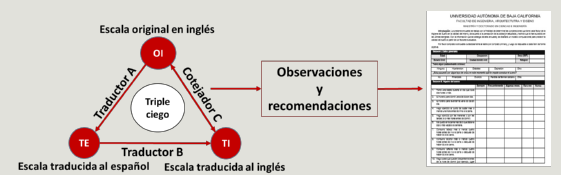
\includegraphics[width=0.8\linewidth]{images/double-translation} 

}

\caption{Double translation}\label{fig:double-tr}
\end{figure}

After this translation, the two questionnaires where joined in a single
questionnaire, adding a section in order to obtain demographic,
emoptional and health data of relevance to this study. The new
questionnaire was comformed by three sections. The first section has six
demographic items, one emotional and one health item, the second section
is the PSQI questionnaire that consists of 20 items, and, the third
section is the SHI whit a total of 21 items. In the end, the SHI survey
was left with 21 items, unlike the original that has 13, this has been,
only for data granularity reasons, however, the changes do not alter the
SHI objective. For example, item six of the original questionnaire that
asked about the use of tobacco, alcohol, or caffeine, became three items
to ask separately about the use of these three substances.

In the end, the questionnaire consisted of 47 items, divided into three
sections that are described later. The purpose of the questionnaire is
to collect data to be analyzed using automated learning techniques
(specifically the techniques of feature selection) to determine those
sleep hygiene factors that have a greater impact on the quality of sleep
from the respondent's perception. One of the specific objectives of this
research is to delimit the domain of input data to a subset of factors
that explain an appropriate percentage of the variance of the
phenomenon. The resulting factors will be used as the predictive
variables in the first stage of training of the inference model to
estimate the quality of sleep.

\subsection{Demographic emotional and health
data}\label{demographic-emotional-and-health-data}

\subsubsection{Demographic}\label{demographic}

In this section we ask about six relevant data that allow to understand
the context of respondent. The six variables are age, gender, ocupation,
kind of work, religion and civil status. Of this six variables,
\textbf{kind of work} provide relevant information to the study, since
the literature says that phisical activity improve the sleep quality
{[}cita{]} . The options for this question are: \emph{intellectual},
\emph{phisical}, \emph{more intellectual than phisical} and, \emph{more
phisical than intellectual}. The other variables in this section are for
exploration purposes regarding of sleep quality and sleep hygiene.

\subsubsection{Emotional}\label{emotional}

This variable asks to the respondent if he/she are in a crisis time. The
crisis can be financial, mourning, divorce, or other that can
significantly alter the quality of sleep. This answer is a target
population filter for this study. Data from people in this circumstances
are noisy to the study and should not be part of the data that will be
used for the analysis.

\subsubsection{Health}\label{health}

Similar than \emph{Emotional} variable, the health variable asks if the
respondent suffers from a chronic degenerative disease such as diabetes,
hypertension, depression or another that can directly or indirectly
alter the quality of sleep. Data from people suffering some disease are
removed before the analysis.

\subsection{Quality of Sleep}\label{quality-of-sleep}

The PSQI is considered the gold standard questionnaire to evaluate
subjective sleep quality \citep{Cameron2010}, and has been used to
estimate the quality of sleep in clinical and nonclinical population
\citep{mastin2006}, and has been referred by numerous researchs in
diverse sleep assessments \citep{bai2012}. This questionnaire evaluates
the quality of sleep using nineteen items grouped in seven components:
subjective sleep quality, sleep duration, sleep latency, sleep
disturbances, use of sleep medication, day time disfunction and sleep
latency. The questionnaire provide a baremo to score each component and
sumarize the final score resulting in a dicotomic varaible; \emph{-good
quality of sleep-} or \emph{-poor quality of sleep-} \citep{psqi1989}.
For the purposes of this study, eighteen of the nineteen items was used
in the second section, it fact does not affect the score results, since
that latter item is not taken into account for the computation of the
scale in the original questionnaire. On the other hand, the last item
has to do with specific sleep disorders, for example, \emph{-sleep
apnea-}, while this study seeks to understand sleep habits in healthy
people.

\subsection{Sleep Hygiene Index}\label{sleep-hygiene-index}

It is an instrument designed to measure the sleep hygiene behavior in a
nonclinical population. Its theoretical basis is in the criteria that
International Classification of Sleep Disorders (ICSD) uses to diagnose
an inadequate sleep hygiene. The scale has thirteen items and has
reported an internal validity of \(\alpha=0.71\), as well a high
reliability in test-retest evaluation\citep{mastin2006}.

For the purposes of this study and based on what the literature reports
regarding sleep hygiene factors, the following adjustments were made to
the instrument, without interfering with its essence:

\begin{itemize}
\item
  Following the structure and the meaning of the item four \emph{- I
  exercise to the point of sweating within 1 h of going to bed-}, two
  items were added: \emph{- I exercise to the point of sweating during
  the morning-} and \emph{-I exercise to the point of sweating during
  the afternoon.- }. The main purpose was to know whether the exercise
  in the morning or in the afternoon is directly correlated with sleep
  quality.{[}cita{]}
\item
  Item six of the original questionnaire that asked about the use of
  tobacco, alcohol, or caffeine, became three items to ask separately
  about the use of these three substances.
\item
  Item 11 in the original questionnaire asks about an uncomfortable
  bedroom, due to four environment factors. In the questionnaire for
  this study, four items was generated from this one.
\item
  Based on what the literature says about dinner type and schedule, and
  its negative impact on sleep quality, an item was added to the
  questionnaire
  \citep[Stefano2014,\citet{Irish2015},\citet{Wentz2011}]{Posner2011}.
\end{itemize}

\section{Validity and reliability}\label{validity-and-reliability}

After the instrument was completed, it was validated by five experts
that qualify each item on a escale of 1 to 5 for two metrics, clarity
and pertinence. All items were qualified as clear and relevant. with the
mean of 4.5 and 4.7 respectively. A sample of 30 people was randomly
selected to perform the pilot test and obtain the internal validity of
the instrument. Cronbach's alpha for the instrument after pilot test was
\(\alpha=0.68\). This \(\alpha\) value is acceptable and consistent with
that reported by \citep{mastin2006} for the SHI scale, with this we
proceeded to apply the questionnaire to a wider population to collect
the dataset with which the analyzes were made for the selection of
Variables that will be taken into account for the construction of the
model.

\section{Dataset}\label{dataset}

As a result of apply the questionnaire, a raw dataset \((m=342, n=47)\)
was obtained, this dataset, have missing data, some columns are no
significant in terms of variance, there exist data in a wrong format to
analyze, among other data quality issues. To obtain the dataset to the
feature selection analysis, it was neccesary a pre-process of data, what
included: The data quality analysis, the data quality plan to attend the
issues and the implementation of the data quality plan. After this
pre-process of data, the final dataset is conformed by one ID, 51
continuous and 10 categorical features grouped as shows the table
\ref{tab:dataset-columns-distribution}.

\begin{table}[ht]
\centering
\caption{Columns distribution by its nature}
\label{tab:dataset-columns-distribution}
\begin{tabular}{lrrr}
\hline
Group             & Categorical & Continuous & Total \\ \hline
ID                & 0           & 1          & 1     \\
Demographics data & 7           & 1          & 8     \\
PSQI              & 14          & 4          & 18    \\
SHI               & 21          & 0          & 21    \\
Scale PSQI        & 8           & 1          & 9     \\
Scale SHI         & 0           & 5          & 5     \\ \hline
Total             & 50          & 12         & 62    \\ \hline
\end{tabular}
\end{table}

The complete description of the dataset is in the tables
\ref{tab:demographic-feature-description},
\ref{tab:psqi-features-description},
\ref{tab:PSQI-Scale-features-description},
\ref{tab:SHI-feature-description} and
\ref{tab:SHI-scale-feature-description}. At the end, the dataset
contains 21 columns of main predictive variables (SHI), one column for
continuous target variable (SQTT), and, one column for categorical
target variable (SQCL). The other features in the dataset have diverse
purposes as the last column of each table describes.

\begin{table}[ht]
    \centering
    \caption{Demographic features description}
    \label{tab:demographic-feature-description}
    \begin{tabular}{|l|l|l|p{5cm}|p{4cm}|}
        \hline
        \multicolumn{1}{|c|}{\textbf{Grupo}} & \multicolumn{1}{c|}{\textbf{Feature}} & \multicolumn{1}{c|}{\textbf{Type}} & \multicolumn{1}{c|}{\textbf{Values}}                                                     & \multicolumn{1}{c|}{\textbf{Purpose}}                              \\ \hline
        ID                                   & EMAIL                                 & Text                               & inf                                                                                      & identificator                                                   \\ \hline
        \multirow{8}{*}{}         & DD1                                   & Continuous                         & {[}1-100{]}                                                                              & \multirow{6}{4cm}{Demographic data for statistical purposes only} \\ \cline{2-4}
        & DD2                                   &        & Female, Male                                                                             &                                                                 \\ \cline{2-2} \cline{4-4} 
        & DD3                                   &                                    & Student, Employer, Teacher, Independent professional, Other                              &                                                                 \\ \cline{2-2} \cline{4-4}
        & DD4                                   & \multirow{6}{*}{Categorical}                                  & Intellectual, Physical, More intellectual than physical, More physical than intellectual &                                                                 \\ \cline{2-2} \cline{4-4} {Demographic}
        & DD5                                   &                                    & SDA, Catholic, Jehovah's withess, Evangelic, Other                                       &                                       \\ \cline{2-2} \cline{4-4} 
        & DD6                                   &                                    & Married, Single, Divorced, Free Union, Other                                             &                                                                 \\ \cline{2-2} \cline{4-5} 
        & DD7                                   &                                    & No, Hypertension, Diabetes, Depression, Other                                            & Demographic information with filtering purposes                 \\ \cline{2-5} 
        & DD8                                   &                                    & No,Financial, Divorce process, Loss of Family, Other                                     & Financial,                                                      \\ \hline
    \end{tabular}
\end{table}

\begin{table}[ht]
    \centering
    \caption{PSQI features description}
    \label{tab:psqi-features-description}
    \begin{tabular}{|l|l|l|p{3cm}|p{5cm}|}
        \hline
        \multicolumn{1}{|c|}{\textbf{Group}} & \multicolumn{1}{c|}{\textbf{Feature}} & \multicolumn{1}{c|}{\textbf{Type}} & \multicolumn{1}{c|}{\textbf{Values}}                    & \multicolumn{1}{c|}{\textbf{Purpose}}                                                                              \\ \hline
        \multirow{18}{*}{PSQI}               & SQ1                                   & \multirow{4}{*}{Continuous}        & A real numer.   $ 0 \leq  SQ1 \leq 12 $                    & \multirow{18}{5cm}{Provide information to PSQI Scale. A 0 value is the best for sleep quality and 3 is the worst} \\ \cline{2-2} \cline{4-4}
        & SQ2                                   &                                    & An integer number. $ 0 \leq SQ2 \leq 60 $               &                                                                                                                 \\ \cline{2-2} \cline{4-4}
        & SQ3                                   &                                    & A real number. $ 0 \leq SQ3 \leq 12 $                      &                                                                                                                 \\ \cline{2-2} \cline{4-4}
        & SQ4                                   &                                    & A real number. $ 0 \leq SQ4 \leq 12 $                      &                                                                                                                 \\ \cline{2-4}
        & SQ5a                                  & \multirow{14}{*}{Categorical}      & \multirow{14}{3cm}{A level variable. $ 0 \leq SQ* \leq 3 $.} &                                                                                                                 \\ \cline{2-2}
        & SQ5b                                  &                                    &                                                         &                                                                                                                 \\ \cline{2-2}
        & SQ5c                                  &                                    &                                                         &                                                                                                                 \\ \cline{2-2}
        & SQ5d                                  &                                    &                                                         &                                                                                                                 \\ \cline{2-2}
        & SQ5e                                  &                                    &                                                         &                                                                                                                 \\ \cline{2-2}
        & SQ5f                                  &                                    &                                                         &                                                                                                                 \\ \cline{2-2}
        & SQ5g                                  &                                    &                                                         &                                                                                                                 \\ \cline{2-2}
        & SQ5h                                  &                                    &                                                         &                                                                                                                 \\ \cline{2-2}
        & SQ5i                                  &                                    &                                                         &                                                                                                                 \\ \cline{2-2}
        & SQ5j                                  &                                    &                                                         &                                                                                                                 \\ \cline{2-2}
        & SQ6                                   &                                    &                                                         &                                                                                                                 \\ \cline{2-2}
        & SQ7                                   &                                    &                                                         &                                                                                                                 \\ \cline{2-2}
        & SQ8                                   &                                    &                                                         &                                                                                                                 \\ \cline{2-2}
        & SQ9                                   &                                    &                                                         &                                                                                                                 \\ \hline
    \end{tabular}
\end{table}

\begin{table}[ht]
    \centering
    \caption{PSQI Scale features description}
    \label{tab:PSQI-Scale-features-description}
    \begin{tabular}{|l|l|l|p{3cm}|p{5cm}|}
        \hline
        \multicolumn{1}{|c|}{\textbf{Group}} & \multicolumn{1}{c|}{\textbf{Feature}} & \multicolumn{1}{c|}{\textbf{Type}} & \multicolumn{1}{c|}{\textbf{Value}}   & \multicolumn{1}{c|}{\textbf{Purpose}}    \\ \hline
        & SQDUR  &   &   & Results of SQ duration. A 0 value is the best for sleep quality and 3 is the worst.                                           \\ \cline{2-2} \cline{5-5} 
        & SQDIS    &      &    & Results of SQ disturbances. A 0 value is the best for sleep quality and 3 is the worst. \\ \cline{2-2} \cline{5-5} 
        \multirow{9}{*}{PSQI Scale} & SQLAT  & \multirow{7}{*}{Categorical}  &  \multirow{7}{3cm}{A level variable. $ 0 < SQ*\leq 3 $.}  & Results of SQ latency. A 0 value is the best for sleep quality and 3 is the worst.    \\ \cline{2-2} \cline{5-5} 
        & SQDD   &    &   & Results of SQ day dysfunction. A 0 value is the best for sleep quality and 3 is the worst. \\ \cline{2-2} \cline{5-5} 
 & SQSE                                  &                                    &                                                       & Results of SQ sleep efficiency. A 0 value is the best for sleep quality and 3 is the worst.                                   \\ \cline{2-2} \cline{5-5} 
        & SQSQ                                  &                                    &                                                       & Results of SQ sleep quality general perception of the respondent. A 0 value is the best for sleep quality and 3 is the worst. \\ \cline{2-2} \cline{5-5} 
        & SQMS                                  &                                    &                                                       & Results of SQ, needs meds. A 0 value is the best for sleep quality and 3 is the worst.                                        \\ \cline{2-5} 
        & SQTT                                  & Continuous                         & An integer value. $ 0 < SQTT\leq 21 $.                 & Total of PSQI                                                                                                                 \\ \cline{2-5} 
        & SQCL                                  & Categorical                        & A level value.                                        & Good/ Poor                                                                                                       \\ \hline
    \end{tabular}
\end{table}

\begin{table}[ht]
    \centering
    \caption{SHI features description}
    \label{tab:SHI-feature-description}
    \begin{tabular}{|l|l|l|l|l|}
        \hline
        \multicolumn{1}{|c|}{\textbf{Group}} & \multicolumn{1}{c|}{\textbf{Feature}} & \multicolumn{1}{c|}{\textbf{Type}} & \multicolumn{1}{c|}{\textbf{Values}} & \multicolumn{1}{c|}{\textbf{Purpose}}   \\ \hline
        \multirow{21}{*}{SHI}  & SHI  & \multirow{21}{*}{Categorical} & \multirow{21}{3cm}{A level variable. $ 0 < SH*\leq 4 $.} & \multirow{21}{5cm}{Predictive Features (Provide information for SHI scale). A 0 value is the best for sleep hygiene and 4 is the worst} \\ \cline{2-2}
        & SH2                                   &                                    &                                                        &                                                                                                                                         \\ \cline{2-2}
        & SH3                                   &                                    &                                                        &                                                                                                                                         \\ \cline{2-2}
        & SH4                                   &                                    &                                                        &                                                                                                                                         \\ \cline{2-2}
        & SH5                                   &                                    &                                                        &                                                                                                                                         \\ \cline{2-2}
        & SH6                                   &                                    &                                                        &                                                                                                                                         \\ \cline{2-2}
        & SH7                                   &                                    &                                                        &                                                                                                                                         \\ \cline{2-2}
        & SH8                                   &                                    &                                                        &                                                                                                                                         \\ \cline{2-2}
        & SH9                                   &                                    &                                                        &                                                                                                                                         \\ \cline{2-2}
        & SH10                                  &                                    &                                                        &                                                                                                                                         \\ \cline{2-2}
        & SH11                                  &                                    &                                                        &                                                                                                                                         \\ \cline{2-2}
        & SH12                                  &                                    &                                                        &                                                                                                                                         \\ \cline{2-2}
        & SH13                                  &                                    &                                                        &                                                                                                                                         \\ \cline{2-2}
        & SH14                                  &                                    &                                                        &                                                                                                                                         \\ \cline{2-2}
        & SH15                                  &                                    &                                                        &                                                                                                                                         \\ \cline{2-2}
        & SH16                                  &                                    &                                                        &                                                                                                                                         \\ \cline{2-2}
        & SH17                                  &                                    &                                                        &                                                                                                                                         \\ \cline{2-2}
        & SH18                                  &                                    &                                                        &                                                                                                                                         \\ \cline{2-2}
        & SH19                                  &                                    &                                                        &                                                                                                                                         \\ \cline{2-2}
        & SH20                                  &                                    &                                                        &                                                                                                                                         \\ \cline{2-2}
        & SH21                                  &                                    &                                                        &                                                                                                                                         \\ \hline
    \end{tabular}
\end{table}

\begin{table}[ht]
    \centering
    \caption{SHI scale feature description}
    \label{tab:SHI-scale-feature-description}
    \begin{tabular}{|l|l|l|p{4cm}|p{4cm}|}
        \hline
        \multicolumn{1}{|c|}{\textbf{Group}} & \multicolumn{1}{c|}{\textbf{Feature}} & \multicolumn{1}{c|}{\textbf{Type}} & \multicolumn{1}{c|}{\textbf{Value}}                    & \multicolumn{1}{c|}{\textbf{Purpose}} \\ \hline
                  & SHSTR                                 &         & Sum of five SH features. $ 0 < SQ*\leq 20 $.           & Group of stress features           \\ \cline{2-2} \cline{4-5} 
        & SHDIS                                 &                                    & Sum of five SH features. $ 0 < SQ*\leq 20 $.           & Group of disruptors features       \\ \cline{2-2} \cline{4-5} 
        \multirow{5}{*}{SHI SCALE} & SHCH          &       \multirow{5}{*}{Continuous}                             & Sum of six SH features. $ 0 < SQ*\leq 24 $.            & Group of circadian features        \\ \cline{2-2} \cline{4-5} 
        & SHDG                                  &                                    & Sum of three SH features. $ 0 < SQ*\leq 12 $.          & Group of drugs features            \\ \cline{2-2} \cline{4-5} 
        & SHTT                                  &                                    & Sum of SHSTR,SHDIS, SHCH and SHDG. $ 0 < SQ*\leq 76 $. & Total of SHI                       \\ \hline
    \end{tabular}
\end{table}

\chapter{Data pre-process}\label{data-pre-process}

\section{Estructuration and validation data
process}\label{estructuration-and-validation-data-process}

Before to generate the quality report of the data, the data are loaded
and passed for a process of validation and restructuration. This process
includes the renaming of the columns and data validation for columns
containing information of time and age. Additionally, the values for the
responses of SHI and PSQI questionnaires was recodified from original
responses (`Nunca',`Casi nunca',`Algunas
veces',`Frecuentemente',`Siempre') to data that can be used to numerical
and algorithmical analysis (`0',`1',`2',`3',`4').

The resulting dataset has 48 columns, distributed as the
\ref{tab:distribution-of-features-by-type} shows:

\begin{table}[ht]
\centering
\caption{Distribution of features in the dataset by type}
\label{tab:distribution-of-features-by-type}
\begin{tabular}{|l|c|l|}
\hline
\multicolumn{1}{|c|}{\textbf{Type}} & \textbf{Quantity} & \multicolumn{1}{c|}{\textbf{Columns in the dataset}} \\ \hline
CharID                              & 1                 & 1                                                    \\ \hline
Categorical                         & 41                & {[}3-9{]} and {[}14-48{]}                            \\ \hline
Continuous                          & 6                 & 2 and {[}10-13{]}                                    \\ \hline
\end{tabular}
\end{table}

The quality analysis of data was based in the recommendations of
\citep{Kelleher2015}. The resulting dataset will allow runs the
algorithms to select the relevant features to generate the model. The
analysis of the data quality includes the treadment of missing values,
outliers and cardinality as well as correction of some possible bugs in
the scripts that do the process of restructuration and validation of the
dataset. The data quality analysis begins with a report of quality of
continouos and categorical features. For continuous variables ten
metrics were analyzed: quantity, missing values, cardinality, minimum
value, first quartile, median, third quartile, maximum value, mean, and
standard deviation. For categorical variables, nine metrics were
analyzed: quantity, missing values, cardinality, mode, mode frequency,
mode percent, second mode, second mode frequency and second mode
percent. Before to do this report, a look at the complete dataset
allowed to identify three records that contains no data for any feature.
These records were deleted to avoid noisy information in the quality
analysis.

\section{Data quality report}\label{data-quality-report}

The data quality report was performed using two scripts, one for
continuous and one for categorical features, so, the features were
grouped by type to do the analysis.

\subsection{Continuous features}\label{continuous-features}

The dataset contains five continuous features, one for demographic data
(DD1=AGE) and four features that measure the sleep duration (SQ1=``Time
to go to bed'', SQ2=``Latency of sleep'', SQ3=``Time to wake up'',
SQ4=``Period of time between going to bed and waking up'').

\begin{table}[ht]
\centering
\caption{Data quality report of continuous features}
\label{tab:data-quality-report-of-continuous-features}
\begin{tabular}{llllllllll}
\hline
\multicolumn{1}{c}{\textbf{Feature}} & \multicolumn{1}{c}{\textbf{Count}} & \multicolumn{1}{c}{\textbf{Miss}} & \multicolumn{1}{c}{\textbf{Card}} & \multicolumn{1}{c}{\textbf{Min}} & \multicolumn{1}{c}{\textbf{Qrt1}} & \multicolumn{1}{c}{\textbf{Median}} & \multicolumn{1}{c}{\textbf{Qrt3}} & \multicolumn{1}{c}{\textbf{Max}} & \multicolumn{1}{c}{\textbf{Mean}} \\ \hline
DD1   & 338  & 6  & 49  & 16    & 27     & 35    & 44      & 66    & 35.92          \\
SQ1   & 338  & 0  & 29  & 0     & 10     & 11    & 11.08   & 12.5  & 9.99           \\
SQ2   & 338  & 1  & 15  & 1     & 5      & 15    & 20      & 60    & 14.99          \\
SQ3   & 338  & 2  & 40  & 0.7   & 5.08   & 6     & 7       & 11    & 6.18           \\
SQ4   & 338  & 3  & 107 & -0.05 & 6.17   & 6.88  & 7.75    & 10.75 & 6.91           \\ 
\hline
\end{tabular}
\end{table}

The table \ref{tab:data-quality-report-of-continuous-features} shows
some irregularities in continuous variables, as we can see, a negative
value is the minimum value in the SQ4 variable; this variable represents
the \emph{Period of time between going to bed and waking up}, thus no
negative value must be enter in this field, likewise, it appear a
\(0.0\) value as the minimun value in the SQ1 variable, which is wrong
because this is the time that respondents said go to bed, and, in this
case, \(0.00\) is not a valid answer, in any case, an appropriate answer
would be \(12.00\), referring to midnight. On the other hand, the
variable SQ2, has a large standard deviation (\(\sigma=11.91\)), since
the variable represents the minutes that person takes to fall asleep in
minutes (\(\mu\simeq 15\)).

No one of these features have a great quantity of missing values, DD1 is
the variable with most of them, however the missing values represents
only the \(0.018 \%\) of the data, whis is not significant. If we assume
that each record that contains a missing value is a different row, we
have \(12\) records, which represents the \(0.036\%\). As this
percentage is small, and there are not in our hands, previous works
describing the tendency of the data, these records with missing values
could be deleted.

These continuos variables shows good cardinality, even though the ratio
between the cardinality and number of records is not close to one. The
nature of the data justifies this fact, because although the features
are continuous and in theory they could take a large number of values,
they take a small range of values, for instance, the variable SQ1 take
an small range of values because the people answer commonly to this kind
of question with onclock time, it means, people ask that they go to bed
at \(9:00\), \(10:30\), \(10:45\) or \(11:00\), even when they, actually
were to bed at \(9:03\), or \(10:33\) referring to the first to
examples. The other variables have similar nature, thus the conclusion
that cardinality is good for this variables, where the smallest
cardinality was 15.

Additionaly to previous analysis, histograms and boxplot were generated
to observe the behaviour of the data.

\begin{figure}[H]

{\centering 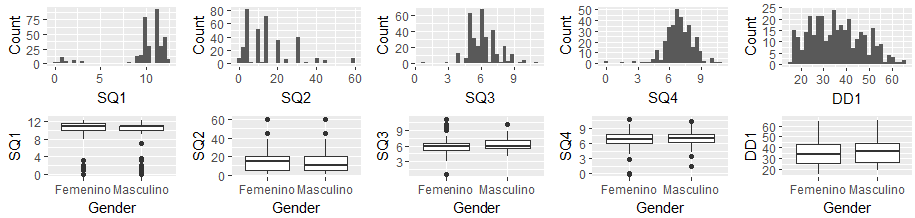
\includegraphics[width=0.9\linewidth]{images/hist-boxplots-continuous-variables} 

}

\caption{Histograms and boxplots of the continuous features}\label{fig:hb-of-cf}
\end{figure}

The plots in the Fig. \ref{fig:hb-of-cf} shows that the continuous
features have outliers which should be analyzed to include/exclude from
de dataset before of the training of the model to obtain better results.
These variables do not intervene directly in the generation of the
model, the model is generated from the SH features, however, these
outliers could be indicators of some disorder of sleep in the
respondent, thus the analysis must be performed.

The Table \ref{tab-data-quality-plan-continuous} summarizes the data
quality issues in continuous features and the potential strategies to
attend them.

\begin{table}[ht]
\centering
\caption{Data quality plan for continuous features}
\label{tab-data-quality-plan-continuous}
\begin{tabular}{|l|p{5cm}|p{8cm}|}
\hline
Feature & Data quality issue  & Strategie \\ \hline
SQ1     & Data contain 0.0, the correct value should be 12.00 & Refine the process of convert data for this field  \\ \hline
SQ4     & Data contain negative values, it is wrong because the data represents the time to wake up & Refine the process validating the data, to correct the problem, or, eliminate the records with this issue. \\ \hline
SQ2     & Standar deviation too large & Finding outliers visually and analytically. Excluding outliers from the modeling may improve the predictions. These analysis of outliers includes all continuous variables.  \\ \hline
All     & Missing values  & The percentage of missing values is low, it allows to eliminate records with missing values. The decision of impute data is a few probable, since no reports are in our bibliography to know the tendency of the data. \\ \hline
\end{tabular}
\end{table}

\section{Categorical Features for demographics
data}\label{categorical-features-for-demographics-data}

The categorical features were divided in two groups, the demographic
features are in the first group and the features containing all the
information over the sleep hygiene are in other group.

\begin{table}[ht]
\centering
\caption{Data quality report of continuous features}
\label{Report-of-quality-of-the-categorical-demographic-features}
\begin{tabular}{llllp{2cm}llp{2cm}ll}
\hline
\textbf{Feat.} & \textbf{Count} & \textbf{Miss} & \textbf{Card} & \textbf{Mode}         & \textbf{MF} & \textbf{M\%} & \textbf{Mode2} & \textbf{M2F} & \textbf{M2\%} \\ \hline
DD2              & 338            & 0             & 2             & Femenino              & 188               & 55.62\%           & Masculino      & 150                & 44.38\%            \\
DD3              & 338            & 1             & 5             & Docente               & 143               & 42.31\%           & Empleado       & 70                 & 20.71\%            \\
DD4              & 338            & 0             & 4             & Más mental que físico & 156               & 46.15\%           & Mental         & 143                & 42.31\%            \\
DD5              & 338            & 2             & 5             & ASD                   & 150               & 44.38\%           & Católica       & 129                & 38.17\%            \\
DD6              & 338            & 0             & 1             & Unión Libre           & 338               & 100\%             & NA             & NA                 & NA\%               \\
DD7              & 338            & 0             & 5             & Ninguno               & 284               & 84.02\%           & Otro           & 26                 & 7.69\%             \\
DD8              & 338            & 1             & 5             & No                    & 272               & 80.47\%           & Otra           & 34                 & 10.06\%            \\ \hline
\end{tabular}
\end{table}

The table
\ref{Report-of-quality-of-the-categorical-demographic-features} shows
only one irregularity in this set of variables, the variable DD6 has the
hihest mode posible (\(100\%\)), if data are right, all respondents are
living in free union status which is very doubtful taken in account the
population were the questionnaire was applied. There are less missing
values than in the continuous features, so, it is possible to think in
eliminate the records. The cardinality is not a problem in this set of
features (except for the variable DD6 as commented above), since all
posibilities have representation. In the two cases (features DD7 and
DD8) where the mode capture a high percentage of the data, the
information is good for this research. DD7 refers to people who suffer
some chronic disease, the best answer to this work is ``Any'' because
the intention is to work with healthy people, likewise in the DD8
variable that ask to the people if they are in some crisis that disrups
their sleep, the best answer to this work is ``No'', fortunatelly, this
is the mode.

\subsection{Categorical features for Slepp
hygiene}\label{categorical-features-for-slepp-hygiene}

\begin{table}[ht]
\centering
\caption{Report of quality of the SH features}
\label{tab:report-of-quality-of-the-sleep-hygiene-features}
\begin{tabular}{llllllllll}
\hline
\multicolumn{1}{c}{\textbf{Feature}} & \multicolumn{1}{c}{\textbf{Count}} & \multicolumn{1}{c}{\textbf{Miss}} & \multicolumn{1}{c}{\textbf{Card}} & \multicolumn{1}{c}{\textbf{Mode}} & \multicolumn{1}{c}{\textbf{MF}} & \multicolumn{1}{c}{\textbf{M\%}} & \multicolumn{1}{c}{\textbf{Mode2}} & \multicolumn{1}{c}{\textbf{M2F}} & \multicolumn{1}{c}{\textbf{M2\%}} \\
\hline
SH1    & 338    & 0   & 5  & 1     & 114   & 33.73\%   & 0   & 111  & 32.84\%  \\
SH4    & 338    & 1   & 5  & 0     & 204   & 60.36\%   & 1   & 67   & 19.82\%  \\
SH5    & 338    & 0   & 5  & 0     & 176   & 52.07\%   & 2   & 64   & 18.93\%  \\
SH6    & 338    & 1   & 5  & 0     & 152   & 44.97\%   & 1   & 75   & 22.19\%  \\
SH7    & 338    & 2   & 5  & 0     & 142   & 42.01\%   & 1   & 107  & 31.66\%  \\
SH8    & 338    & 0   & 5  & 0     & 319   & 94.38\%   & 4   & 7    & 2.07\%   \\
SH9    & 338    & 0   & 4  & 0     & 276   & 81.66\%   & 1   & 34   & 10.06\%  \\
SH10   & 338    & 0   & 5  & 0     & 223   & 65.98\%   & 1   & 57   & 16.86\%  \\
SH11   & 338    & 1   & 5  & 0     & 104   & 30.77\%   & 2   & 78   & 23.08\%  \\
SH12   & 338    & 0   & 5  & 1     & 133   & 39.35\%   & 2   & 114  & 33.73\%  \\
SH13   & 338    & 0   & 5  & 2     & 92    & 27.22\%   & 1   & 76   & 22.49\%  \\
SH14   & 338    & 0   & 5  & 0     & 210   & 62.13\%   & 1   & 61   & 18.05\%  \\
SH15   & 338    & 1   & 5  & 0     & 101   & 29.88\%   & 1   & 91   & 26.92\%  \\
SH16   & 338    & 0   & 5  & 0     & 163   & 48.22\%   & 1   & 84   & 24.85\%  \\
SH17   & 338    & 1   & 5  & 0     & 222   & 65.68\%   & 1   & 82   & 24.26\%  \\
SH18   & 338    & 0   & 5  & 0     & 173   & 51.18\%   & 1   & 82   & 24.26\%  \\
SH19   & 338    & 0   & 5  & 0     & 125   & 36.98\%   & 1   & 81   & 23.96\%  \\
SH20   & 338    & 0   & 5  & 2     & 117   & 34.62\%   & 1   & 90   & 26.63\%  \\
SH21   & 338    & 0   & 5  & 1     & 130   & 38.46\%   & 2   & 96   & 28.40\%  \\ 
\hline
\end{tabular}
\end{table}

In Table \ref{tab:report-of-quality-of-the-sleep-hygiene-features}, the
cardinality shows that all possible value \([0-5]\) for each answer is
represented in the data, except by the SH9 variable where one of the
options was not selected as answer of the respondents. It is good for
the quality of data, however, there are two variables with high mode.
The 81.66 \% of the respondents, answered \emph{never (\(0\))} to the
question SH9 \emph{``I use alcohol within 4 hours of going to bed or
after going to bed.''}, while the 94.38\% answered \emph{never (\(0\))}
to the question SH8 \emph{``I use tobacco within 4 hours of going to bed
or after going to bed.''}, which means that there are few variability in
the data in these two variables. It is possible to dispense with these
data for the analysis, since they do not contribute much information to
the studied phenomenon for this population. The other 19 categorical
variables for SHI, have a cardinality of 5, and the higher mode is
placed in SH10 \emph{``I use cafeine within 4 hours of going to bed or
after going to bed.''} were a \(66.98\%\) of the respondents answered
\emph{never (\(0\))} for this question. This means that the answers have
a good range of variability to be analized, and to participate as
candidate of be selected as feature to training the model.

This set of data has small number of missing values, however, in this
case it is possible to impute data due to the features together
represents a behavior of the person. Algorithms as KNN or a multiple
logistic regression can performs data imputation to have a good
approximation to the true data. The table
\ref{Tab:Potential-strategies-to-attend-SH-features} present the summary
of the issues and potential strategies for the SH features.

\begin{table}[ht]
\centering
\caption{Potential strategies to attend SH features}
\label{Tab:Potential-strategies-to-attend-SH-features}
\begin{tabular}{|l|p{4cm}|p{8cm}|}
\hline
Feature & Data quality issue  & Strategie  \\ 
\hline
SH8 & The mode is very high (\textgreater94\%) & Analyze the relevance of include this variable to the analysis due the few variability   \\ 
\hline
SH9 & The mode is high (\textgreater81\%)      & Analyze the relevance of include this variable to the analysis due the few variability \\ 
\hline
All & Missing values                           & The percentage of missing values is small, however, imputation will be performed for this missing values. \\ 
\hline
\end{tabular}
\end{table}

\section{Following the quality plan to attend
issues}\label{following-the-quality-plan-to-attend-issues}

The first step in order to attend the issues was the analysis of the
code that validates the raw data, to avoid the suspicious of bugs that
could be generate wrong data. After the code is validated, the errors in
data can be adjudicate to human capture.

After the analysis of scripts, tree bugs were fixed. The first bug is
related with the reason that the civil status have a mode equivalent to
the number of records in the dataset. The bug was generated by
omittining a condition in the evaluation of a missing value in the field
in the same line of code that attempt to standardize the results so that
all the sentences were in the same style of case. In the case of status
civil feature, some answers are wroten as \emph{`Unión libre'}, while
other was wroten as \emph{`Unión Libre'}.

The line with the bug:

\texttt{ifelse(is.na(dataSet\$DD6),dataSet\$DD6\textless{}-NA,dataSet\$DD6\textless{}-"Unión\ Libre")}

The line after being fixed:

\texttt{ifelse(is.na(dataSet\$DD6),dataSet\$DD6\textless{}-NA,dataSet{[}dataSet\$DD6==\textquotesingle{}Unión\ libre\textquotesingle{},7{]}\textless{}-"Unión\ Libre")}

The second bug was identified in the script that calculates the time of
sleep depending of the three variables, \emph{`Time to go the bed'},
\emph{`Time to wake up'}, \emph{`Time to fall asleep'}, in this case,
the condition for the calculation does not contemplate that a person
could say that he went to bed and got up twelve hours apart. The problem
was solved by modifying the conditional operator of \(>\) to \(\geq\).

Code with bug:

\begin{verbatim}
  if(HD>HL){
    HD<-HD-12.00
  }
  SE<-abs(HL-HD)
  SE<-SE-round(minutos/60,digits = 2)
\end{verbatim}

Code after being fixed:

\begin{verbatim}
  if(HD>=HL){
    HD<-HD-12.00
  }
  SE<-abs(HL-HD)
  SE<-SE-round(minutos/60,digits = 2)
\end{verbatim}

The third bug was corrected by adding two condition per values before
ignored. Values in the range of \((-\infty,0)\) must be taken a NA
value, and values in the range of \([0,1)\) must be transformed by
adding 12.00.

The lines that were added are:

\begin{verbatim}
  if(!is.na(s3)){
    if(as.numeric(s3)<0){
      s3<-NA
    }else if(as.numeric(s3)<1){
      s3=as.numeric(s3)+12
    }else{
      s3<-as.numeric(s3)
    }
  }
\end{verbatim}

The quality reports generated after apply this corrections, show a
difference in the identified features with possible issues due to a
wrong treatment.

\begin{table}[ht]
\centering
\caption{Quality report of continuous features after recoding the scripts}
\label{tab-quality-report-continuous-after-recoding-scripts}
\begin{tabular}{lllllllllll}
\hline
\multicolumn{1}{c}{\textbf{Feature}} & \multicolumn{1}{c}{\textbf{Count}} & \multicolumn{1}{c}{\textbf{Miss}} & \multicolumn{1}{c}{\textbf{Card}} & \multicolumn{1}{c}{\textbf{Min}} & \multicolumn{1}{c}{\textbf{Qrt1}} & \multicolumn{1}{c}{\textbf{Median}} & \multicolumn{1}{c}{\textbf{Qrt3}} & \multicolumn{1}{c}{\textbf{Max}} & \multicolumn{1}{c}{\textbf{Mean}} & \multicolumn{1}{c}{\textbf{Sdev}} \\ 
\hline
DD1   & 338  & 6  & 49  & 16  & 27    & 35  & 44    & 66    & 35.92    & 11.41     \\
SQ1   & 338  & 0  & 27  & 1   & 10    & 11  & 11.5  & 12.75 & 10.17    & 2.46      \\
SQ2   & 338  & 1  & 15  & 1   & 5     & 15  & 20    & 60    & 14.99    & 11.91     \\
SQ3   & 338  & 2  & 40  & 3   & 5.21  & 6   & 7     & 12.7  & 6.21     & 1.33      \\
SQ4   & 338  & 3  & 107 & 0.12& 6.17  & 6.89& 7.75  & 11.95 & 6.94     & 1.33      \\ 
\hline
\end{tabular}
\end{table}

\begin{table}[ht]
\centering
\caption{Quality report of demographic features after recoding the scripts}
\label{tab-quality-report-demographic-after-recoding-scripts}
\begin{tabular}{llllp{2cm}lllll}
\hline
\multicolumn{1}{c}{\textbf{Feature}} & \multicolumn{1}{c}{\textbf{Count}} & \multicolumn{1}{c}{\textbf{Miss}} & \multicolumn{1}{c}{\textbf{Card}} & \multicolumn{1}{c}{\textbf{Mode}} & \multicolumn{1}{c}{\textbf{MF}} & \multicolumn{1}{c}{\textbf{M\%}} & \multicolumn{1}{c}{\textbf{Mode2}} & \multicolumn{1}{c}{\textbf{M2F}} & \multicolumn{1}{c}{\textbf{M2\%}} \\ \hline
DD2   & 338  & 0   & 2    & Femenino                  & 188   & 55.62\%  & Masculino      & 150  & 44.38\%  \\
DD3   & 338  & 1   & 5    & Docente                   & 143   & 42.31\%  & Empleado       & 70   & 20.71\%  \\
DD4   & 338  & 0   & 4    & Más mental que físico     & 156   & 46.15\%  & Mental         & 143  & 42.31\%  \\
DD5   & 338  & 2   & 5    & ASD                       & 150   & 44.38\%  & Católica       & 129  & 38.17\%  \\
DD6   & 338  & 0   & 5    & Casada(o)                 & 181   & 53.55\%  & Soltera(o)     & 119  & 35.21\%  \\
DD7   & 338  & 0   & 5    & Ninguno                   & 284   & 84.02\%  & Otro           & 26   & 7.69\%   \\
DD8   & 338  & 1   & 5    & No                        & 272   & 80.47\%  & Otra           & 34   & 10.06\%  \\ \hline
\end{tabular}
\end{table}

The minimum value in SQ1 is not zero as before, now it is one, which is
reasonable; the variable SQ4 do not have a negative value as minimum
value. The present also is very small (\(0.12\)) and was verified in the
raw data, the conclusion is that it was a wrong user capture, the
respondent said that he/she go to bed at 12:30 and wakes up at 12:42
every day. On the other hand, the civil status (DD6) has a congruent
value for the sample of study, the \(53.55\%\) of the respondents said
be married and \(35.21\%\) be single, in contrast with previous data
where it was reported that \(100\%\) of the people had a `Free union'
civil status.

The second step was to work with the missing values in the continuous
features and missing values in the categorical demographic features.
Records containing missing values were eliminated as proposed in the
data qulaity plan described in Table
\ref{tab-data-quality-plan-continuous}. The same apply to the
categorical demographic features.

After applying the process to delete records with missing values in
continuous and categorical demographics features the dataset reducts its
dimentionality from 338 to 326, which represents a reduction of 0.036\%
of the original data.

In the third step of this stage the atypical values are identified to
exclude them from the dataset that will serve as a source of the
training of the model. The process excludes records that exceed three
standard deviations in the variable SQ4 (`time the person spent
asleep'). This variable is of high impact on the quality of sleep and is
not considered within the factors of sleep hygiene. Another indicator of
a possible sleep disorder is the latency, latency is the time between a
person go to bed and he/she fall asleep. The records containing outliers
in this feature, also were eliminated.

After delete records with outliers n continuous variables the dataset
reducts its dimentionality from 338 to 306, which represents a reduction
of 0.095\% of the original data.

The Fig. \ref{fig:hb-of-cf-after-deloutliers}, shows the histograms and
boxplots after eliminated records with outliers in SQ2 and SQ4, boxplots
in these two variables make it clear that do not outliers were found for
these features. DD1 has no outliers too, even though maintaining the
original records.

\begin{figure}[H]

{\centering 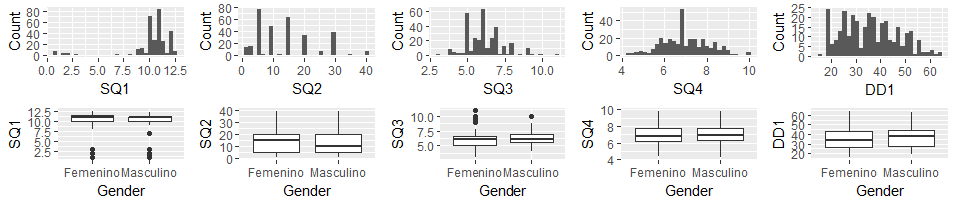
\includegraphics[width=0.9\linewidth]{images/hist-boxplots-continuous-variables-after-delete-outliers} 

}

\caption{Histograms and boxplots of the continuous features after delete outliers}\label{fig:hb-of-cf-after-deloutliers}
\end{figure}

\section{Imputation of missing values in SH and SQ
features}\label{imputation-of-missing-values-in-sh-and-sq-features}

The process of imputation was performed using \emph{mice and VIM
package} \citep[\citet{VIM2016}]{mice2011}. the process begins with the
analysis of missing values in the variables involved indirectly or
directly in the generation of the model. The table
\ref{tab-report-of-missing-value-in-SHSQ} shows that the dataset has few
missing values (Not all columns in the table are included for lack of
space, however, all columns that were omitted do not have missing
values). It has \(297\) complete records, a record with a missing value
in the column SQ5a, one more with a missing value in the column SQ5c, an
so on. The dataset contains eight records with a total of nine missing
values in eight variables.

\begin{table}[ht]
\centering
\caption{Report of missing values}
\label{tab-report-of-missing-value-in-SHSQ}
\begin{tabular}{|l|l|l|l|l|l|l|l|l|l|l|l|l|l|l|}
\hline
    & SQ5b & SQ5d & ... & SH20 & SH21 & SQ5a & SQ5c & SH4 & SH6 & SH11 & SH15 & SH17 & SH7 &   \\ \hline
297 & 1    & 1    & ... & 1    & 1    & 1    & 1    & 1   & 1   & 1    & 1    & 1    & 1   & 0 \\ \hline
1   & 1    & 1    & ... & 1    & 1    & 0    & 1    & 1   & 1   & 1    & 1    & 1    & 1   & 1 \\ \hline
1   & 1    & 1    & ... & 1    & 1    & 1    & 0    & 1   & 1   & 1    & 1    & 1    & 1   & 1 \\ \hline
1   & 1    & 1    & ... & 1    & 1    & 1    & 1    & 0   & 1   & 1    & 1    & 1    & 1   & 1 \\ \hline
1   & 1    & 1    & ... & 1    & 1    & 1    & 1    & 1   & 0   & 1    & 1    & 1    & 1   & 1 \\ \hline
2   & 1    & 1    & ... & 1    & 1    & 1    & 1    & 1   & 1   & 1    & 1    & 1    & 0   & 1 \\ \hline
1   & 1    & 1    & ... & 1    & 1    & 1    & 1    & 1   & 1   & 0    & 1    & 1    & 1   & 1 \\ \hline
1   & 1    & 1    & ... & 1    & 1    & 1    & 1    & 1   & 1   & 1    & 0    & 1    & 1   & 1 \\ \hline
1   & 1    & 1    & ... & 1    & 1    & 1    & 1    & 1   & 1   & 1    & 1    & 0    & 1   & 1 \\ \hline
    & 0    & 0    & ... & 0    & 0    & 1    & 1    & 1   & 1   & 1    & 1    & 1    & 2   & 9 \\ \hline
\end{tabular}
\end{table}

A summary of the missing values its presented in the table
\ref{summary-of-missing-values-SH}

\begin{table}[ht]
\centering
\caption{Summary of missing values in SH features}
\label{summary-of-missing-values-SH}
\begin{tabular}{|l|l|}
\hline
Feature & Count of missing values \\ \hline
SQ5a    & 1                       \\ \hline
SQ5b    & 1                       \\ \hline
SH4     & 1                       \\ \hline
SH6     & 1                       \\ \hline
SH7     & 2                       \\ \hline
SH11    & 1                       \\ \hline
SH15    & 1                       \\ \hline
SH17    & 1                       \\ \hline
Total   & 7                       \\ \hline
\end{tabular}
\end{table}

The figure \ref{fig:f-pattern-of-missing-data} shows in the left side,
an histogram of the features with missing data depicting the influence
of missing values in the dataset. The right side shows the pattern of
missing values in the dataset, it concentrates all complete cases in the
botton of the graph, which reach a 97.06\% of the dataset. The remaining
of the figure shows the features with missing data, placing in the right
side the corresponding percentages per variable.

\begin{figure}[H]

{\centering 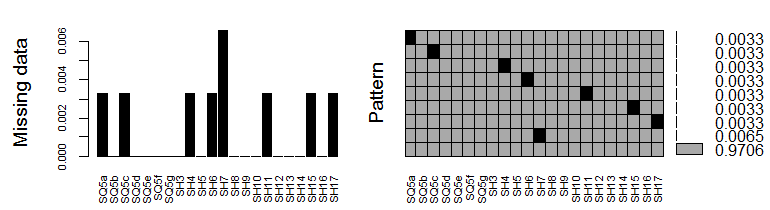
\includegraphics[width=0.9\linewidth]{images/pattern-of-missing-data} 

}

\caption{Pattern of missing values}\label{fig:f-pattern-of-missing-data}
\end{figure}

The \emph{mice} function was executed to impute data in the records
containing missing values, the process was performed in a temporal
dataset comformed only for those features with missing data. The
\emph{mice} function perform data imputation using \emph{polytomous
regression imputataion} for unordered categorical data with more of two
leves, which is the case. The multinomial logistic regression was
applied with 50 iterations and five datasets to obtain a table of
results that allow to choose the best option to do the imputation.

\begin{table}[ht]
\centering
\caption{Five datasets with data imputation}
\label{datasets-of-impute-data}
\begin{tabular}{|l|l|l|l|l|l|}
\hline
Number of Row & DS1 & DS2 & DS3 & DS4 & DS5 \\ \hline
ROW 225       & 2   & 1   & 0   & 1   & 3   \\ \hline
ROW 72        & 3   & 1   & 0   & 2   & 2   \\ \hline
ROW 12        & 0   & 0   & 0   & 0   & 3   \\ \hline
ROW 233       & 2   & 1   & 1   & 4   & 2   \\ \hline
ROW 17        & 0   & 1   & 2   & 1   & 0   \\ \hline
ROW 146       & 0   & 1   & 2   & 0   & 2   \\ \hline
ROW 144       & 3   & 0   & 0   & 3   & 1   \\ \hline
ROW 183       & 0   & 4   & 0   & 3   & 4   \\ \hline
ROW 201       & 0   & 2   & 0   & 0   & 0   \\ \hline
\end{tabular}
\end{table}

The DS4 is the dataset most consistent with the proposals in the other
datasets, it matches with at least one dataset of the remaining four, in
seven of the rows. The DS4 was chosen to impute data in these variables.

\begin{table}[ht]
\centering
\caption{Report of missin gvalues after imputation}
\label{tab-report-of-missingvalues-after-imputation}
\begin{tabular}{lllllllll}
SQ5a & SQ5c & SH4 & SH6 & SH11 & SH15 & SH17 & SH7 &   \\
1    & 1    & 1   & 1   & 1    & 1    & 1    & 1   & 0 \\
0    & 0    & 0   & 0   & 0    & 0    & 0    & 0   & 0
\end{tabular}
\end{table}

The table \ref{tab-report-of-missingvalues-after-imputation}, shows that
no missing value are in the dataset after the imputation, now the new
dataset of variables with data imputation will be merged with the others
features of the original dataset in a new dataset to be saved and used
in advanced to train the model.

\section{Final results}\label{final-results}

The following tables show the report of quality in the dataset after
apply deletion of missing values, exclusion of records containing
outliers and imputation of missing values in variables that are closely
related with the training of the model.

\begin{table}[ht]
\centering
\caption{Report of Quality of SH features after cleaning and imputation}
\label{tab-report-of-quality-of-sh-features}
\begin{tabular}{|l|l|l|l|l|l|l|l|l|l|}
\hline
Feature & Count & Miss & Card & Mode & ModeFrec & ModePerc & Mode2 & Mode2Frec & Mode2Perc \\ \hline
SH1     & 306   & 0    & 5    & 1    & 109      & 35.62\%  & 0     & 97        & 31.70\%   \\ \hline
SH2     & 306   & 0    & 5    & 1    & 109      & 35.62\%  & 2     & 107       & 34.97\%   \\ \hline
SH3     & 306   & 0    & 5    & 1    & 147      & 48.04\%  & 2     & 70        & 22.88\%   \\ \hline
SH4     & 306   & 0    & 5    & 0    & 186      & 60.78\%  & 1     & 63        & 20.59\%   \\ \hline
SH5     & 306   & 0    & 5    & 0    & 159      & 51.96\%  & 2     & 56        & 18.30\%   \\ \hline
SH6     & 306   & 0    & 5    & 0    & 135      & 44.12\%  & 1     & 69        & 22.55\%   \\ \hline
SH7     & 306   & 0    & 5    & 0    & 128      & 41.83\%  & 1     & 99        & 32.35\%   \\ \hline
SH8     & 306   & 0    & 5    & 0    & 292      & 95.42\%  & 3     & 5         & 1.63\%    \\ \hline
SH9     & 306   & 0    & 4    & 0    & 254      & 83.01\%  & 1     & 30        & 9.80\%    \\ \hline
SH10    & 306   & 0    & 5    & 0    & 201      & 65.69\%  & 1     & 53        & 17.32\%   \\ \hline
SH11    & 306   & 0    & 5    & 0    & 95       & 31.05\%  & 2     & 69        & 22.55\%   \\ \hline
SH12    & 306   & 0    & 5    & 1    & 122      & 39.87\%  & 2     & 99        & 32.35\%   \\ \hline
SH13    & 306   & 0    & 5    & 2    & 85       & 27.78\%  & 1     & 69        & 22.55\%   \\ \hline
SH14    & 306   & 0    & 5    & 0    & 188      & 61.44\%  & 1     & 54        & 17.65\%   \\ \hline
SH15    & 306   & 0    & 5    & 0    & 94       & 30.72\%  & 1     & 80        & 26.14\%   \\ \hline
SH16    & 306   & 0    & 5    & 0    & 150      & 49.02\%  & 1     & 76        & 24.84\%   \\ \hline
SH17    & 306   & 0    & 5    & 0    & 200      & 65.36\%  & 1     & 78        & 25.49\%   \\ \hline
SH18    & 306   & 0    & 5    & 0    & 158      & 51.63\%  & 1     & 73        & 23.86\%   \\ \hline
SH19    & 306   & 0    & 5    & 0    & 112      & 36.60\%  & 1     & 78        & 25.49\%   \\ \hline
SH20    & 306   & 0    & 5    & 2    & 107      & 34.97\%  & 1     & 85        & 27.78\%   \\ \hline
SH21    & 306   & 0    & 5    & 1    & 122      & 39.87\%  & 2     & 88        & 28.76\%   \\ \hline
\end{tabular}
\end{table}

With exception of high percentages in mode of the SH8 and SH9, all other
features present a good behavior in the dataset. The issue of SH8 and
SH9 will be attended in a future stage of the work, the process of
feature selection will take care of this.

The last process to be carried out in this stage is the calculation of
SHI and PSQI scores through the scales provided by the respective
questionnaires.

The final dataset to be used in the process of feature selection is a
306 x 62 dataset containing 10 continuous features, 51 categorical
features and one ID feature. To more detail of this dataset, see please
the tables at the end of the previous section.

\chapter{Methods}\label{methods}

We describe our methods in this chapter.

\chapter{Applications}\label{applications}

Some \emph{significant} applications are demonstrated in this chapter.

\section{Example one}\label{example-one}

\section{Example two}\label{example-two}

\chapter{Final Words}\label{final-words}

We have finished a nice book.

\bibliography{packages,book}


\end{document}
